\documentclass[10pt,a4paper]{article}
%You comment with the modulo-sign. Before the \begin keyword you put what packages
%you want to use etc. If you want to include graphics for example you need the graphicX-package
\usepackage{graphicx}
\usepackage{amsmath}
\usepackage{float}
%You also define your title here. You create a title by putting maketitle after you have begun the document
\title{Requirements Specification}
\author{\begin{large}{Robot group}\end{large}\\\\
Olle Fridolfsson (ollfr940) \\  Niklas Hansson (nikha310) \\ Patrik Hillgren (pathi747) \\ Benjamin Ingberg (benin542)\\ Par Lundgren (parlu048) \\ Mattias Nilsson (matni796)}
\setlength{\parindent}{0cm}	%This removes the automatic indentation
\begin{document}
\maketitle
%Latex keeps track of your sectioning automatically. To get a table of contents just put
\newpage
\tableofcontents
%To get a new page just put
\newpage
\noindent %Just makes it so that the first paragraph isn't indented
\section{Introduction}
This document will specify the requirements for the Robotics Safety project that is a part of the course TSBB11 at LiU, held at CVL. The project is done upon a request from Yaskawa Nordic AB, located in Torsås, as the they wish to use the result for inspiration and further analysis of similar applications.
\section{Purpose and goal}
The purpose of the project is to develop a system that monitors the surroundings of industrial robots and allows humans to safely work side-by-side with them. 
The goal is to provide a system that meets the expectation of Yaskawa Nordic AB.
The requirements of the project are all assigned to different sprints. The sprints are not definitive but can be changed depending on how much time the different requirements take to fulfill. 

\section{Definitions}
There are predefined safety zones for the surrounding of the robot and these will be used to decide whether the robot should continue to work as normal, slow down its working pace or simply stop.

\section{System Overview}
The system will consist of at least one kinect sensor that monitors the robot and sends data containing information from the robot and it’s surroundings to a computer. Together with data from the controller, which describes the robots position, it is possible to detect if anything “human-like” is entering the region of interest.

\begin{figure}[H] 
  \centering
    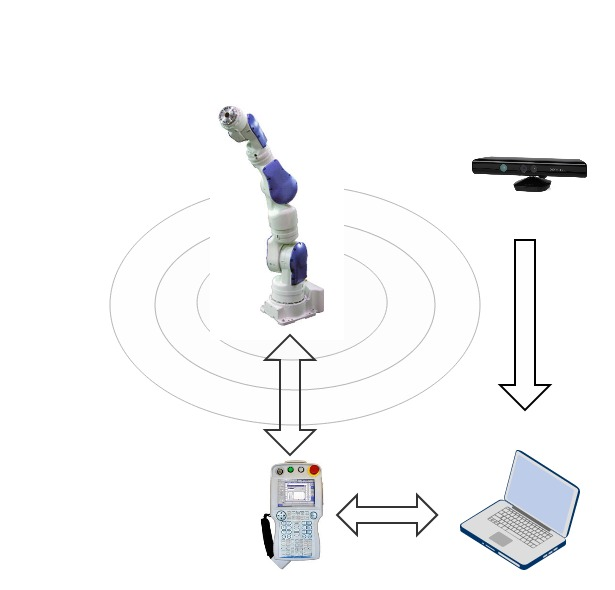
\includegraphics[width = 0.7\textwidth]{robot.jpg}
    \caption{A picture of the robot, the kinect camera and the connecting computer.}
    \label{fig:safetyzone}
\end{figure}


\section{Requirements}
The requirements of the project are listed below. If a requirement is planned to be solved in specific sprint, it is marked with the number of that sprint. 
{\addtolength{\leftskip}{5mm}
\subsection{Product Requirements}
This section describes the requirements of the finished product. These are the overall goals of the project. \par}

\begin{enumerate}
\item Control of the robots working pace with respect to the closest human being, sprint 3.

{\addtolength{\leftskip}{5mm}The robot will slow down if a human being is approaching it and stop if someone gets to close.\par}

\item Evaluation of the products performance and reliability using an automatic system, sprint 4.

\subsection{System Interfaces}
These section describes how the functionality of the of the program will be split into modules.

\item There will be a module for tracking using statistical background models, sprint 2.

{\addtolength{\leftskip}{5mm}It will be important to know what in the Kinect image which is background and what is objects. To know this some kind of tracking is needed. In this project statistical background modelling will be used.\par}
\item There will be a module for generating a 3D-model from robot data,\\ sprint 2.
 
{\addtolength{\leftskip}{5mm}The robot will give information about it’s orientation. This module will take that information and generate a 3D model of it.\par}
 
 \item There will be a module for linking data from 3D model of robot and results from tracking, sprint 3.

{\addtolength{\leftskip}{5mm}This module distinguishes the robot from other moving objects in the images.\par}

\item There will be a module for evaluation of system, sprint 4.

{\addtolength{\leftskip}{5mm}This module will compute distances to humans, gives an accuracy measurement feedback and displays the number of moving objects in the environment. 
\par}

\item There will be a module for controlling robot, sprint 3.

{\addtolength{\leftskip}{5mm}The robot will be controlled based on moving objects within the safety zones. This module will manage this, sending the correct signals to the robot based on what is found in the depth and color image.
\par}

\item There will be a module for Real-time visualization of all 3D data,\\ sprint 3.

{\addtolength{\leftskip}{5mm}There will be an interactive environment where the robot and other 3D data is visualized. Combined or separate.\par}

\subsection{Hardware Interfaces}

\item Camera setup specifications, sprint 2.

{\addtolength{\leftskip}{5mm} The number of cameras and their positions will be specified.\par}

\subsection{Communication Interfaces}

\item Data from the Kinect sensor available in the computer, sprint 1.
\item Data from the robot controller in the computer, sprint 1.

\subsection{Constraints assumptions and dependencies}
These are the requirements that is assumed to be fulfilled for the system being able to work properly. None of them are categorized to a sprint.

\item The robot will not be occluded from the point of view of the camera.

\item The Kinect sensor should be placed in a position so that it can overview the robot from above. That ensures that a human being not will be able to approach the robot without entering the safety zones.

\item The system will not work in a pitch black environment, there is an assumption of a reasonable amount of light.

\item The data used will always be the current input from camera and robot, i.e there will not be any module handling delays between inputs.

\subsection{Functional requirements}
This section describes the requirements of functionality for the subsystems and for the system in general.
\item Process information from Robot controller and generate 3D data, \\sprint 2.
\item Send control signal to the Robot from computer, sprint 2.
\item Link the robots 3D data to the 3D data from the Kinect sensor, sprint 3.

\item Determine the distance from the robot to the other found objects, \\sprint 3.

\item Evaluate the performance of the result automatically, sprint 4.

\item Detect a human being that is entering the area of interest, sprint 4.

\item Track objects in the image using statistical background models, sprint 2.

\subsection{Documentation requirements}
This section describes which documents will be written by the group. The deadline of the document is also specified.
\item Design Specification, 24/9, Sprint 1.
\item Project Plan, 24/9, Sprint 1.
\item Requirement Specification, 24/9, Sprint 1.
\item Technical documentation of the project,13/12  Sprint 4.
\item Summary of the completed backlog after every sprint.
\item Web-page displaying the results, 13/12, Sprint 4.




\end{enumerate}

\end{document}

